\documentclass{../template/labo}
\usepackage[utf8x]{inputenc}

\usepackage[frenchb]{babel}
\usepackage[T1]{fontenc}

\usepackage{graphicx}
\usepackage{amssymb}
\usepackage{amsmath}
\usepackage{wasysym} %smiley
\usepackage{hyperref}% hyperliens
\usepackage{tikz}
\usetikzlibrary{babel,positioning,calc}
\usepackage[]{circuitikz}
\usepackage{textcomp}
% \usepackage{minted}
\usepackage[long]{datetime}
\usepackage{gensymb} % \ohm, celsius
\usepackage{framed}
\usepackage{pdfpages}
\usepackage{todo}
\usepackage{paralist}
\usepackage{multicol}

\usepackage{mathastext} % math as standfard text : units are respecting typography conventions.
\usepackage{fancyhdr} %en-tête
\usepackage{qrcode}

\langexam{frenchb}

\correction{false}
 %\correction{true}

\author{The Fantastic Four}


%% fancy header & foot
\pagestyle{fancy}
\lhead{[ELEC-H-301] Électronique appliquée\\ LABO \no 2 : Conception et réalisation d'un amplificateur audio\ifthenelse{\boolean{corrige}}{~-- corrigé}{}}
\rhead{v2.0.0\\ page \thepage}
\cfoot{}
%%

\pdfinfo{
/Author (Raoul Sommeillier, ULB -- BEAMS)
/Title (LABO 2 ELEC-H-301, Conception et réalisation d'un amplificateur audio)
/ModDate (D:\pdfdate)
}

\hypersetup{
pdftitle={LABO 2 [ELEC-H-301] Électronique appliquée: Conception et réalisation d'un amplificateur audio},
pdfauthor={ ULB - BEAMS  },
pdfsubject={Conception et réalisation d'un amplificateur audio}
}

%\date{\vspace{-1cm}\mydate\today}
%\title{\vspace{-2cm} Labo \no 6\\ Électronique appliquée [ELEC-H-301]\\Réalisation d'un ampli à transistor\ifthenelse{\boolean{corrige}}{~\\Corrigé}{}}

%\author{\vspace{-1cm}}%\textsc{Yannick Allard}}

\setlength{\parskip}{0.5cm plus4mm minus3mm} %espacement entre §
\setlength{\parindent}{0pt}


\begin{document}

\tptitle{}{Séance 2~: Conception et réalisation d'un amplificateur audio}

\section{But de la manipulation}

Les buts de cette manipulation sont :
\begin{itemize}
	\item illustrer l'utilisation des amplificateurs opérationnels dans une application réaliste ;
	\item réaliser un montage électronique « grand public ».
\end{itemize}

\section{Pré-requis}
Les notions liées aux amplis-op sont supposées connues :
\begin{itemize}
\item adaptation d'impédances ;
\item gain ;
\item produit gain-bande passante ;
\item imperfections.
\end{itemize}
En particulier, vous devez être capable de résoudre des problèmes semblables à ceux des séances d'exercices n°2 et 3.

\section{Matériel}
En plus du matériel classique de laboratoire (multimètre, oscilloscope, générateur de fonction, câbles, etc.), cette séance nécessite les composants suivants:
\begin{itemize}
\item Ampli-ops (AOP): 4 AOP TLE2061 et 1 NJM2113 (JRC-K002A).
\item Résistances : 1 de $1k\Omega$, 2 de $2,7k\Omega$, 4 de $22k\Omega$, 1 de $39k\Omega$, et 2 de $100k\Omega$.
\item Potentiomètres : 3 de $100k\Omega$.
\item Condensateurs : 2 de $100nF$, 1 de $330nF$, et 1 de $1\mu F$.
\item Un haut-parleur, un câble jack et un protoboard.
\end{itemize}

\textbf{Note :} Il est \textbf{déconseillé} de prendre tous les composants au début du laboratoire. Construisez un étage à la fois et ne prenez que les composants utiles pour ce dernier.

\newpage
\section{Prédéterminations} %{\normalsize{(1 point)}}}
Avant d'entrer au laboratoire, il est conseillé de lire le dimensionnement du montage (§\ref{Dimensionnement}) et de comprendre le
fonctionnement du montage. Revoir les séances d'exercices n°2 et 3 est également une bonne idée.

\section{Objectifs}
A la fin de ce laboratoire, vous devez  :
\vspace{3mm}
\begin{itemize}
\item être capable d'expliquer le fonctionnement de notre ampli audio ;
\item être capable de câbler proprement un circuit complexe sur un protoboard ;
\item vous être rendu compte qu'on peut comprendre le fonctionnement d'un circuit électronique complexe en identifiant des blocs (étages ampli-op, filtres) et en les analysant séparément, pour après comprendre le fonctionnement de l'ensemble.
\end{itemize}



\section{Manipulation}
\subsection{Définition du problème}
Le but de ce laboratoire est de réaliser une chaîne d'amplification audio.
La source sera fournie par la sortie audio d'un ordinateur ou de votre téléphone via le connecteur jack 3.5 mm.
\textit{Note : }Étant donné que cette sortie est déjà amplifiée, afin qu'on puisse par exemple y connecter une paire d'écouteurs, nous allons artificiellement dégrader le signal à l'aide d'un diviseur résistif.

On dispose des informations suivantes :
\vspace{3mm}
\begin{itemize}
\item Vous devez régler votre source pour qu'elle produise un signal d'environ 25 mV crête à la sortie du diviseur résistif, avec une impédance de sortie d'environ $100k\Omega$.
\item Le HP se comporte comme une résistance de $16\Omega$ dans la plage des fréquences audio (impédance classique d'un HP). Sa puissance est limitée à 500 mW.
\item La plage des fréquences audio s'étend de 20 Hz à 20 kHz.
\item On désire pouvoir régler le volume sonore.
\end{itemize}


\subsection{Dimensionnement de l'ampli audio}
\label{Dimensionnement}

\subsubsection{Définition des critères de dimensionnement de l'ampli}

\begin{itemize}
\item Impédance d'entrée : $Rin >> 100k\Omega$
\item impédance de sortie : $Rout << 16\Omega$
\item gain : pour pouvoir régler le volume sonore, nous aurons besoin d'un gain variable. Cherchons le gain maximum nécessaire :
\item le gain minimum doit idéalement valoir 0 pour pouvoir annuler totalement le volume, ce qui implique la présence d'au moins un étage inverseur dans notre montage.
\item bande passante : la bande passante de chaque étage doit être supérieure ou égale à 20kHz.
\end{itemize}

\Question
{
Calculez la valeur de crête maximum supportée par le HP.
}
{}
\Question
{
Déduisez-en le gain maximum du montage.
}
{}

\subsubsection{Calcul du nombre d'étages nécessaire}
Nous utiliserons donc des TLE2061P (ou des TL081) pour ce montage.
\Question
{
Calculez le gain maximum d'un étage à TLE2061P qui respecte la bande passante voulue.
}
{}
\Question
{
Déduisez-en le nombre d'étages nécessaires pour notre ampli audio.
}
{}


\subsubsection{Choix du type des étages}
\Question
{
Le 1er étage doit être un étage non inverseur. Expliquez pourquoi.
}
{}

Le choix du deuxième étage est moins strict, nous choisirons le montage inverseur pour pouvoir annuler totalement le gain.

On peut diviser le gain entre les deux étages librement (tant qu'on ne dépasse le gain maximum pour un étage) ; on a choisi 40 pour le premier étage et 4 pour le second.

On obtient donc un 1er schéma pour notre ampli audio :
\begin{center}
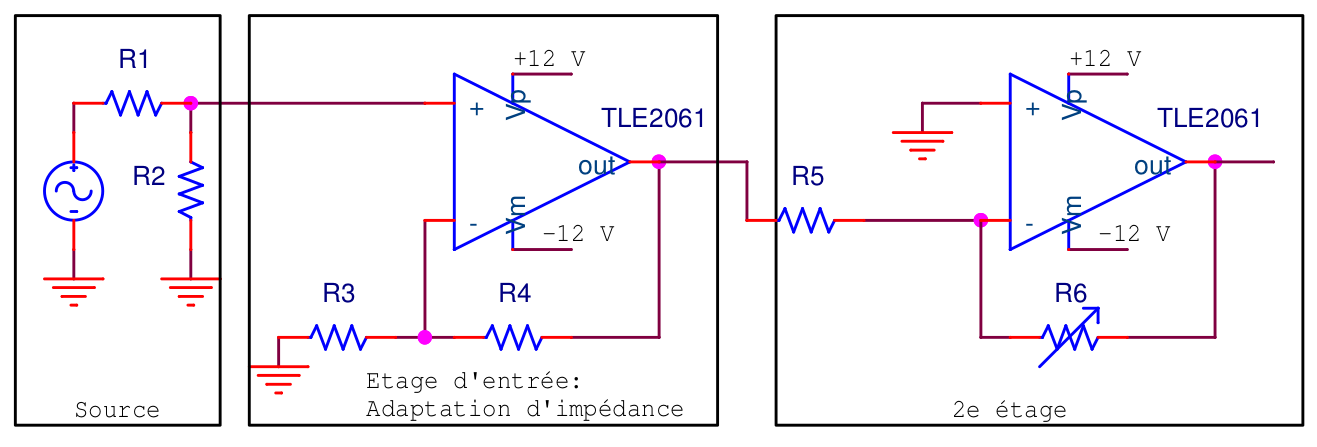
\includegraphics[width=14cm]{figures/AOP2etages.png}
\end{center}
Avec les composants suivants~:
\begin{center}
\begin{tabular}{|c||c||c||c||c||c|}\hline
$R_1 = 10 k\Omega$ & $R_2 = 100 k\Omega$ & $R_3 = 1 k\Omega$ & $R_4 = 39 k\Omega$ & $R_5 = 22 k\Omega$ & $R_6 = 100 k\Omega$ \\ \hline
\end{tabular}
\end{center}

\textit{Note :} En pratique, nous utiliserons une résistance de $22 k\Omega$ dans le deuxième étage, valeur bien plus commune que $25 k\Omega$. Le gain de cet étage sera donc de 4.54 au lieu de 4 comme dimmensionné.

Le potentiomètre $R_6$ est utilisé comme résistance variable et nous permet ainsi de faire varier le gain total du montage de 0 à 160 (181 en réalité).

\subsubsection{Effet des imperfections}

\Question
{
Calculez l'effet des tensions de décalage d'entrée des deux amplis-op sur la tension de sortie.
\textit{Note :} Pour cette question, on ignore donc la contribution des courants de polarisation et de décalage, ainsi que la contribution de la source de tension.
}
{}
\Question
{
Vérifiez que l'effet des courants d'entrée est négligeable.
}
{}
Les HP ne supportent pas qu'on leur applique des tensions continues ; en effet, la partie électrique d'un HP est essentiellement composée d'une bobine dont l'impédance est quasi nulle en continu. Il faudra donc éliminer cette composante continue.

\subsubsection{Étage de sortie}
On peut remarquer que la résistance de charge est de faible valeur ; cela implique qu'il faut pouvoir lui fournir un courant important :
$$I_{out,max}=\frac{V_{out,max}}{R_{H.P.}}=\frac{4V}{16\Omega}=250mA$$
C'est beaucoup plus que ce que peut fournir un TLE2061P. Il faut donc ajouter un 3e étage, appelé étage de sortie, dont le rôle est de fournir le courant nécessaire à la charge. Il existe des amplis-op spécialement conçus pour réaliser ces étages de sortie.\\
Les fabricants conseillent d'utiliser ces amplis-op dans des montages dont le gain est faible (typiquement A = 1), pour optimiser leurs performances. Leur but n'est pas d'amplifier leur tension d'entrée, mais de fournir le courant
nécessaire à la charge.

On utilisera l'ampli-op NJM2113 (JRC-K002A) ; il peut fournir une puissance de 400 mW à une charge de $16\Omega$. Il a été spécialement conçu pour les applications demandant une faible puissance sonore : GSM, baladeur, carte son, etc.

Malheureusement, ces appareils ne disposent en général que d'une source de tension de 5V (produite en régulant la tension de la batterie ou des piles) ; il est impossible d'alimenter les ampli-op de manière symétrique (+12V/- 12V, +5V/-5V, etc). Le NJM2113 a donc été spécialement conçu pour être alimenté en +5V/0V.\\
Cela a une conséquence importante (et gênante) : les limites d'écrêtage de l'ampli ne sont plus symétrique et en particulier, le signal de sortie ne peut plus devenir négatif.\\
On ne peut donc pas amplifier directement notre signal (qui est purement alternatif) avec cet ampli.\\
On doit lui ajouter une composante continue, pour que le signal de sortie ne devienne jamais négatif :
\begin{center}
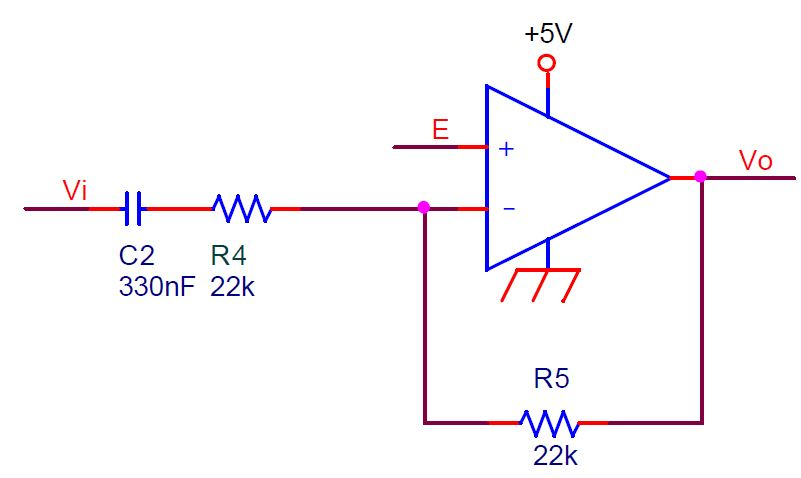
\includegraphics[width=10cm]{figures/AOPetage3}
\end{center}

Dans le schéma ci-dessus, $V_i$ est le signal que l'on veut amplifier (signal utile) et $E$ est une tension continue (à déterminer) qui va empêcher la tension de sortie de devenir négative.\\
On a ajouté un condensateur en série avec l'entrée, pour supprimer l'éventuelle composante continue de $V_i$. Cet étage a donc un comportement de filtre passe-haut; sa fréquence de coupure est de $20Hz$.
\Question
{
Calculez l'effet de $E$ sur la tension de sortie, sachant que $E$ est une tension purement continue.
}
{}
\Question
{
Calculez l'effet de $V_i$ sur la tension de sortie, en considérant que $V_i$ est une tension purement continue.
}
{}
\Question
{
Calculez l'effet de $V_i$ sur la tension de sortie, en considérant que $V_i$ est une tension sinusoïdale dont la fréquence est telle qu'on peut considérer que $C2$ comme un court-circuit.
}
{}
\Question
{
Ce montage est un filtre passe-haut. Vérifiez que sa fréquence de coupure vaut environ $20Hz$.
}
{}

On doit choisir la valeur de $E$ qui maximise l'amplitude admissible de $V_i$ ; il faut donc choisir $E = 2,5V$ pour avoir une valeur crête de $V_i = 2,5V$.\\
Avec ce montage, on arrive donc à amplifier notre signal d'entrée sans être gêné par les limites d'écrêtage de l'ampli-op.\\
Ce montage a cependant un gros inconvénient : sa tension de sortie a une composante continue importante ($2,5V$); on ne peut donc connecter directement un HP à sa sortie. On pourrait placer un condensateur entre la sortie de l'ampli et le HP pour créer un filtre passe-haut, mais la valeur de ce condensateur devrait être très élevée pour avoir une fréquence de coupure de $20Hz$ :
$$C=  \frac{1}{2 \pi R_{H.P.}f_C}=995\mu F$$

$1mF$ est une valeur de capacité qui n'est pas irréaliste, mais qui est à la limite de ce qui est réalisable. Un condensateur de $1mF$ se présente typiquement sous la forme d'un cylindre de 1 à 2cm de diamètre et de 4cm de hauteur; il s'agit donc d'un élément volumineux, peu adapté pour être inclus dans un appareil portable.\\
Les concepteurs du NJM2113 ont donc imaginé une astuce pour éviter de devoir utiliser un tel condensateur :
\begin{center}
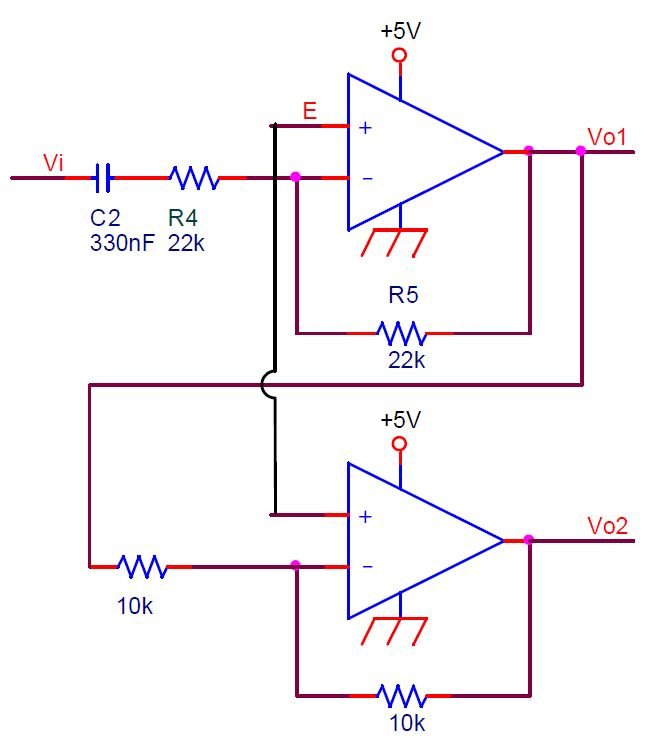
\includegraphics[width=10cm]{figures/AOPetage32}
\end{center}

\Question
{
Vérifiez que : $V_{o1}=E-V_i$ et $V_{o2}=E+V_i$ tel que $V_o=V_{o2}-V_{o1}=2V_i$
}
{}

En plaçant notre HP entre les sorties des deux amplis, on lui applique une tension purement alternative : puisque -les deux tensions de sortie ont la même composante continue, ces dernières s'annulent.\\
Le circuit NJM2113 intègre presque toute cette solution :
\begin{center}
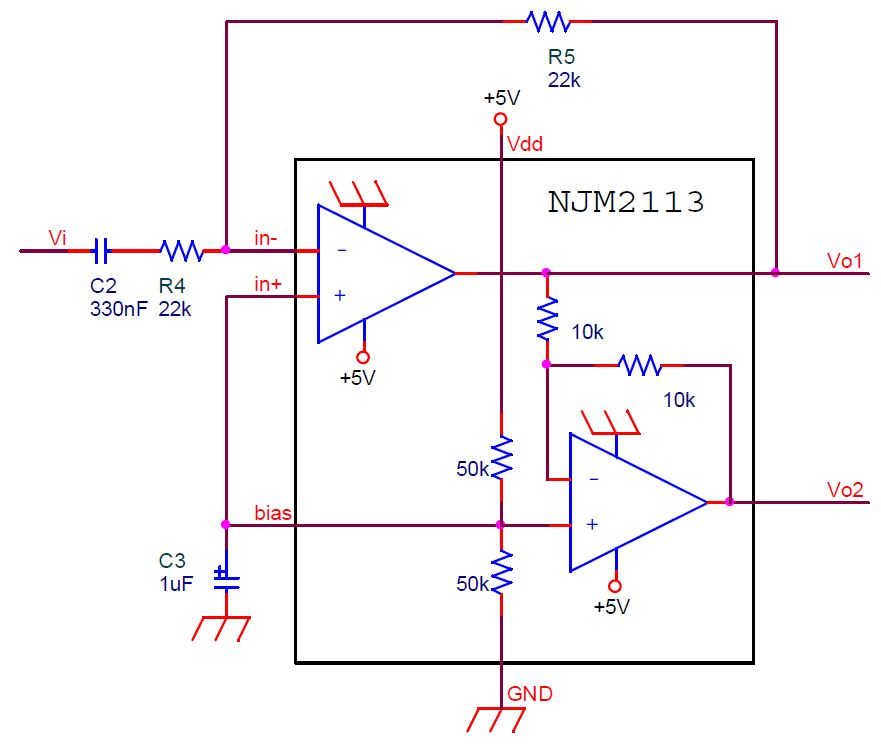
\includegraphics[width=10cm]{figures/NJM}
\end{center}

Le circuit intégré (partie encadrée) contient : les 2 amplis-op, les résistances de rétroaction du 2e ampli et un diviseur résistif pour créer la tension continue $E$ de $2,5V$.\\
Nous devons ajouter à l'extérieur : les résistances de rétroaction du 1er ampli, le condensateur du filtre passe-haut et un condensateur de grande valeur en parallèle sur la tension continue de $2,5V$ ($C3$). Ce condensateur sert à stabiliser la tension continue (il forme un filtre passe-bas avec le diviseur résistif).\\
Le schéma complet de notre ampli audio devient :
\begin{center}
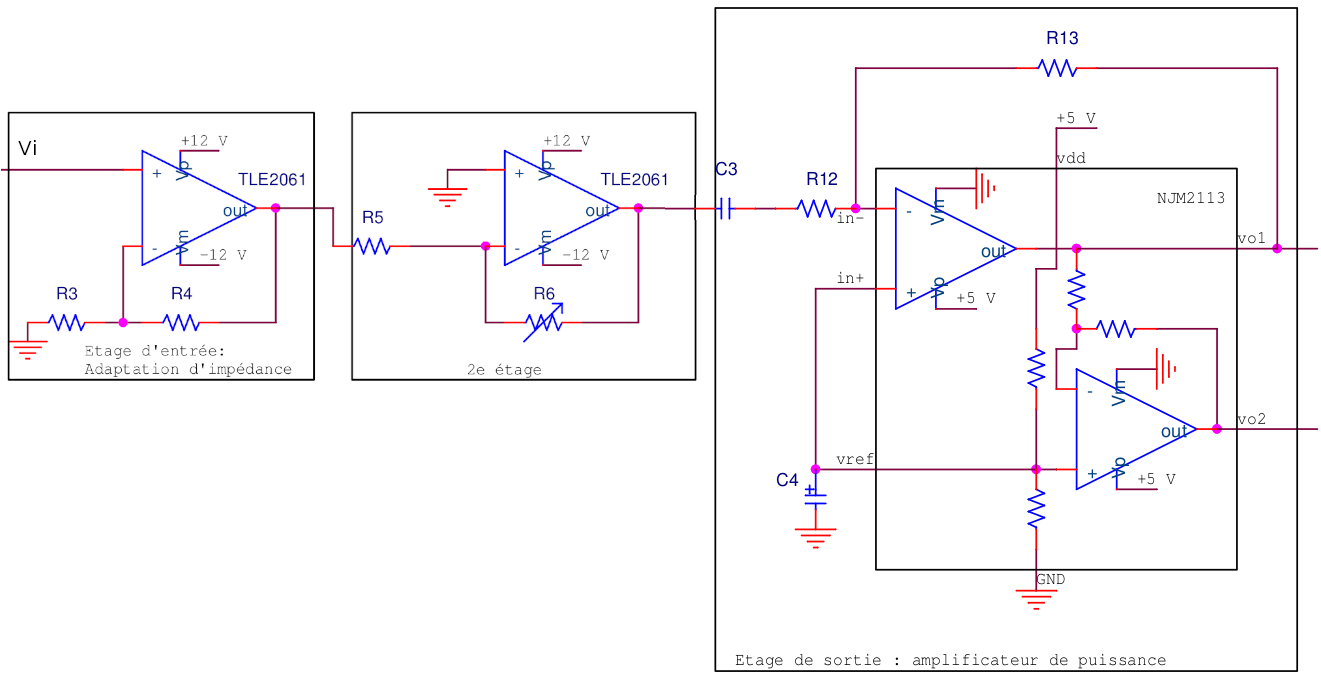
\includegraphics[width=16cm]{figures/montage_complet_sans_bassesaigus.png}
\end{center}

\subsubsection{Ajout d'un contrôle basses/aigus}
Nous avons à présent un amplificateur capable d'amplifier un signal dans la gamme audio avec un gain variable de $0$ à $160$, et de fournir la puissance nécessaire à notre HP, sans risque de le détruire.\\
Nous pouvons encore améliorer notre montage en lui ajoutant un contrôle basses/aigus.\\
Pour pouvoir amplifier différemment les basses et les aigus, il faut d'abord les séparer; cela se fait au moyen de deux filtres : un filtre passe-bas et un filtre passe-haut (filtres RC).\\
Ensuite, on amplifie chacun des deux signaux obtenus à la sortie des filtres avec un étage amplificateur à gain variable entre $0$ et $1$.\\
Finalement, on « remélange » les deux signaux avec un montage sommateur :
\begin{center}
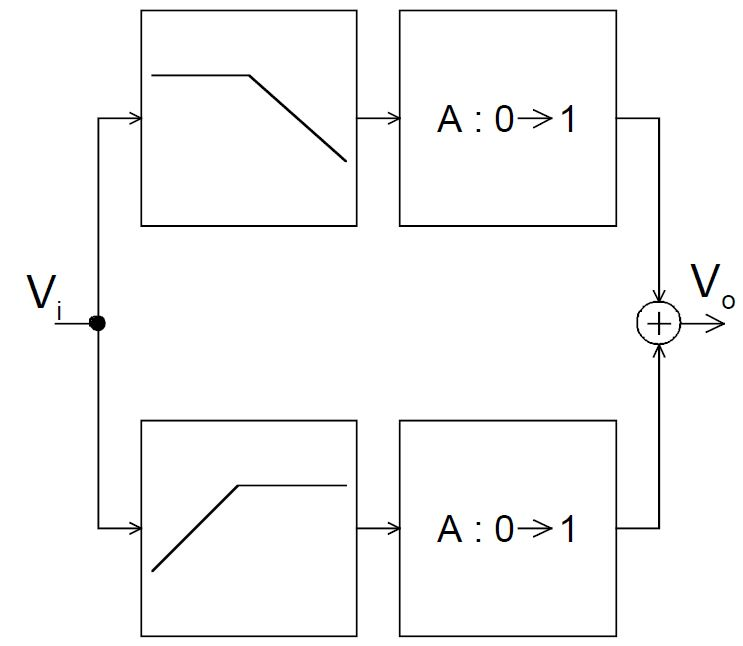
\includegraphics[width=7cm]{figures/AOPsommateur}
\end{center}

Il faut choisir la position de ce contrôle dans notre montage; il y a priori 4 emplacements possibles : avant l'étage d'entrée, avant le 2e étage, avant l'étage de sortie et avant le HP.

\Question
{
Expliquez lesquelles de ces solutions sont bonnes et pourquoi.
}
{}

On a choisi de placer notre égaliseur avant le 2e étage.
Il reste à choisir la fréquence de coupure de nos deux filtres ; la première idée qui vient à l'esprit est de placer la fréquence de coupure au milieu de la bande audio, pour la diviser en deux parts égales.
C'est une bonne idée, mais il y a une subtilité : l'oreille humaine possède une sensibilité logarithmique de la fréquence.

Pour s'en persuader, il suffit de regarder les fréquences des notes de musique.
Elles sont organisées en octaves; une octave comprend 12 tons, également espacés; ils correspondent aux 12 touches d'un piano :
\begin{center}
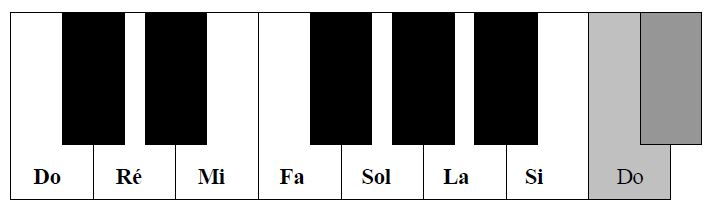
\includegraphics[width=10cm]{figures/AOPpiano}
\end{center}

Le tableau ci-dessous donne les fréquences des notes de musique (en $Hz$), pour 2 octaves consécutives :
\begin{center}
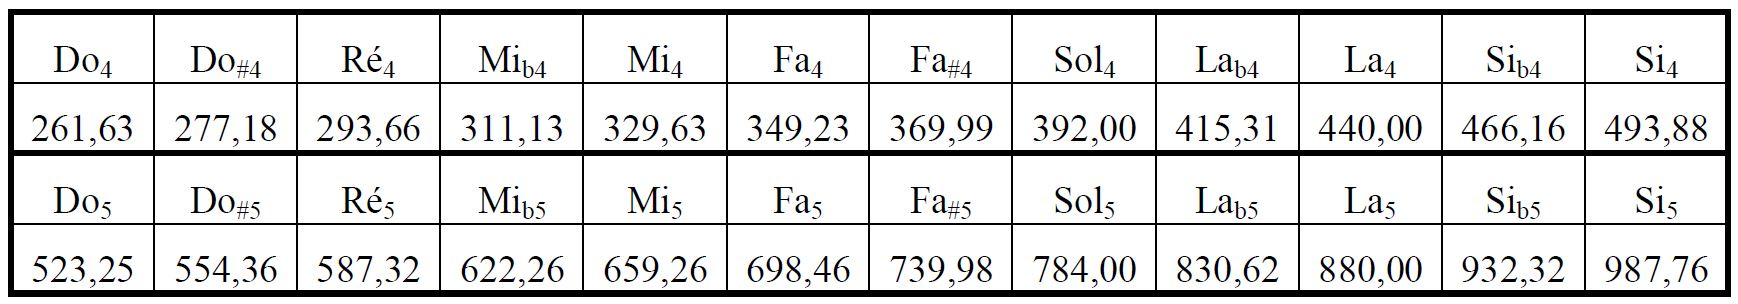
\includegraphics[width=16cm]{figures/AOPpianotable}
\end{center}

Le $La_4$ est la note sur laquelle on accorde les instruments; c'est aussi celle que vous entendez lorsque vous décrochez votre téléphone. On voit que d'une octave à l'autre, la fréquence de chaque note a été multipliée par $2$. La fréquence des notes de musique forme une suite géométrique de raison $\sqrt[12]{2}$.\\
Les bonnes oreilles humaines entendent les notes depuis le $Do_0$ ($16,35Hz$) jusqu'au $Do_{10}$ ($16742Hz$), soit $10$ octaves.\\
De ceci, on peut déduire que la fréquence séparant les basses des aigus doit être la moyenne géométrique (et non la moyenne arithmétique) des fréquences extrêmes de la gamme audio, soit le $Do_5$.

Le schéma de notre contrôle basses/aigus est donc :
\begin{center}
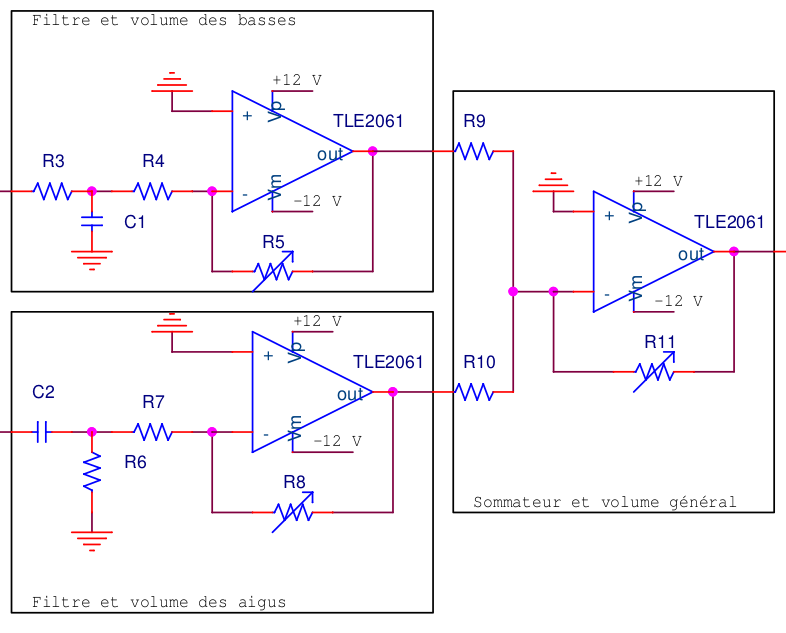
\includegraphics[width=12cm]{figures/egaliseur_sommateur.png}
\end{center}

Pour expliquer son fonctionnement, prenons le bloc Filtre + volume des basses :
\begin{center}
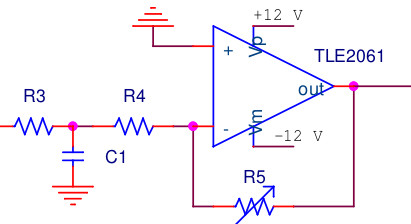
\includegraphics[width=8cm]{figures/AOPfiltrebasse}
\end{center}
Il s'agit en fait de deux blocs mis en cascade : un filtre RC passe-bas et un ampli inverseur.
Pour calculer la fréquence de coupure du filtre, il faut tenir compte de l'impédance d'entrée de l'ampli :
\begin{center}
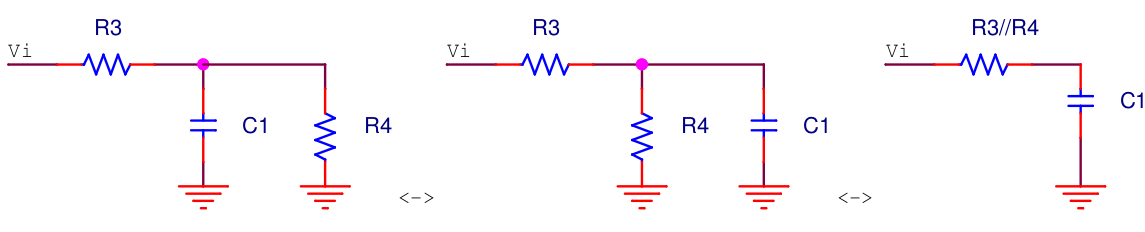
\includegraphics[width=14cm]{figures/filter.png}

\begin{tabular}{|c||c||c|}\hline
$R_3 = 2.7 k\Omega$ & $R_4 = 100 k\Omega$ & $C_1 = 100 nF$ \\ \hline
\end{tabular}
\end{center}


La fréquence de coupure est donc $605Hz$.
L'ampli inverseur nous permet d'avoir un gain variable entre $0$ et $1$ (avec un déphasage de $180^{o}$).
Le mélange des deux signaux obtenus se fait en transformant le 2e étage en sommateur. On peut remarquer qu'il n'est pas nécessaire de placer une capacité en série avec l'entrée du signal des aigus dans le sommateur puisqu'il est déjà passé par un filtre passe-haut.

\subsubsection{Schéma final}
Le schéma final de notre amplificateur audio est donné à la page suivante.

\subsection{Manipulation}
\Question
{
Réalisez, sur protoboard, l'ampli audio que nous avons dimensionné ci-dessus.
\textit{Note :} Utilisez une sinusoïde issue du générateur comme source de tension dans un premier temps.
}
{}

\Question
{
Observez que $V_{o1}$ et $V_{o2}$ simultanément sur les deux canaux de l'oscilloscope et remarquez qu'ils ont bien la même composante continue et des composantes alternatives en opposition de phase.\\
\textbf{ATTENTION}, vous ne pouvez pas observer $V_{o2} - V_{o1}$ sur un seul canal de l'oscilloscope. Pourquoi ?
}
{}

\Question
{
Mettez les contrôles des basses et des aigus au maximum (position neutre), et relevez la fonction de transfert de votre ampli en utilisant le générateur de fonction comme source.\\
Le cahier des charges est-il respecté ?
}
{}

\Question
{
Relevez les fréquences de coupure des filtres aigus et basses (en plaçant le volume de l'autre filtre sur $0$).
}
{}

\Question
{
Branchez le HP et votre source à votre ampli. Ecoutez l'effet du contrôle basses/aigus.
}
{}
\begin{minipage}{.7\textwidth}
\begin{center}
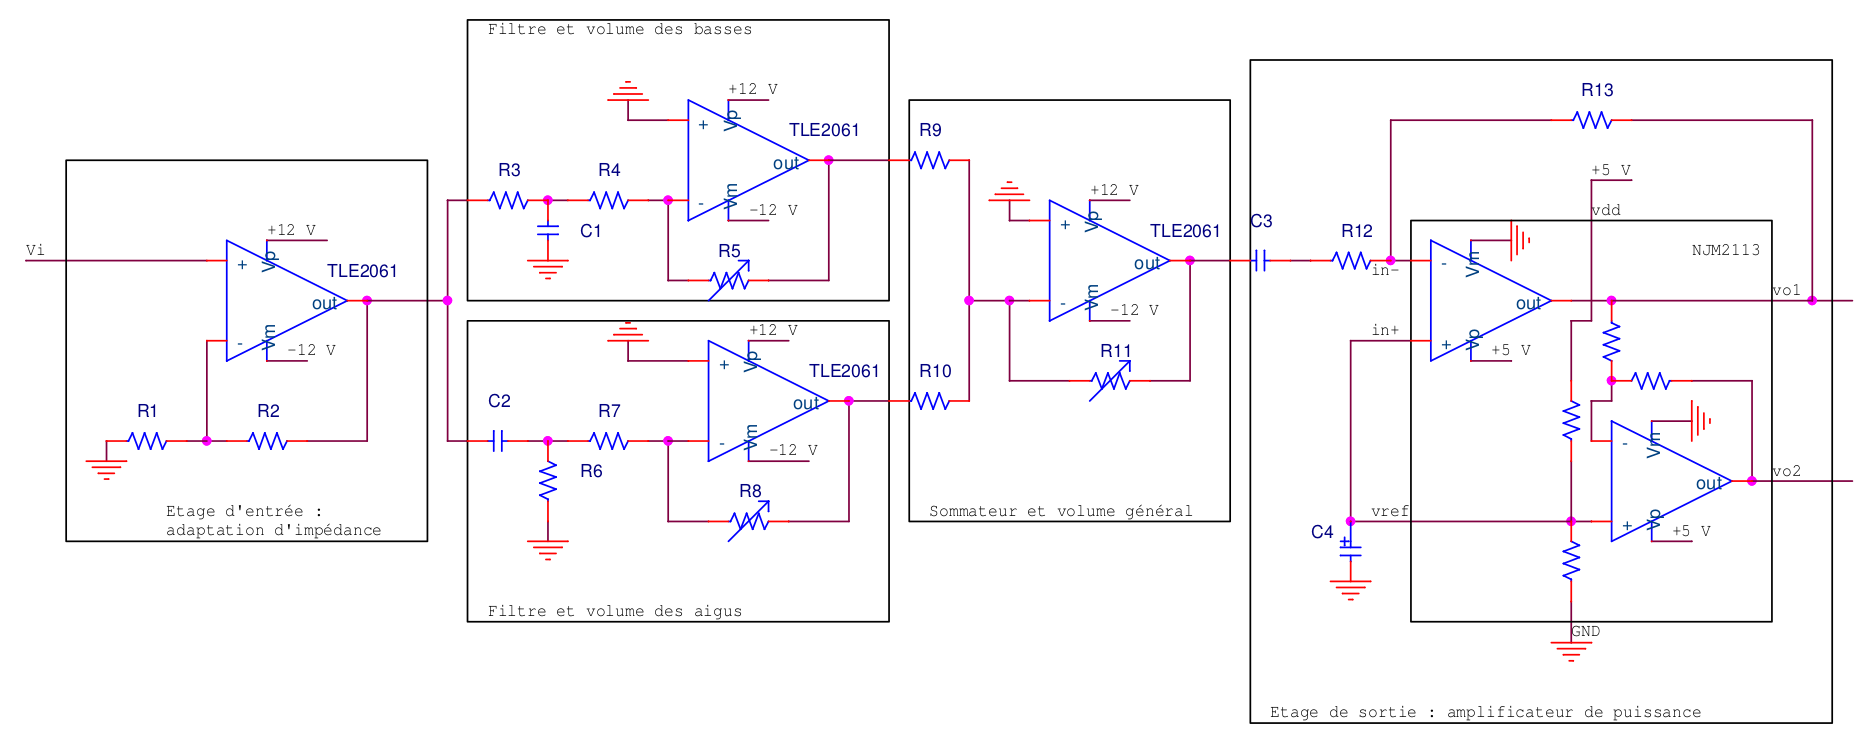
\includegraphics[width=26cm, angle=90]{figures/montage_complet.png}
\end{center}
\end{minipage}
\begin{minipage}{.25\textwidth}
\begin{center}
\rotatebox{90}{
\begin{tabular}{|c|c|c|c|c|c|}\hline
$R_1 = 1 k\Omega$ & $R_2 = 39 k\Omega$ & $R_3 = 2.7 k\Omega$ & $R_4 = 100 k\Omega$ & $R_5 = 100 k\Omega$ & $R_6 = 2.7 k\Omega$ \\ \hline
$R_7 = 100 k\Omega$ & $R_8 = 100 k\Omega$ & $R_9 = 22 k\Omega$ & $R_{10} = 22 k\Omega$ & $R_{11} = 100 k\Omega$ & $R_{12} = 22 k\Omega$ \\ \hline
$R_{13} = 22 k\Omega$ & $C_1 = 100 nF$ & $C_2 = 100 nF$ & $C_3 = 330 nF$ & $C_4 = 1 \mu F$ & \\ \hline
\end{tabular}
}
\end{center}
\end{minipage}

\end{document}
